\documentclass[11pt]{article}
\usepackage{icmlko}
\begin{document}

\title{축을 두 배로 늘려도 틈이 그대로다 --- 개수를 양쪽에서 뺀다}
\author{월드모델 실험실}
\date{노트 438 · 2026년 8월 6일}
\maketitle

\begin{abstract}
노트 435 · 436 · 437이 연달아 같은 처방에 이르렀다 --- \emph{축이 다섯이 아닌
집 밖 도메인이 있어야 두 요인을 가른다.} 새로 모으는 대신 \textbf{KR 만화에
축을 붙였다}: 레코드에 \texttt{start\_date} 가 있으니 달력 축 여섯이
계산되고(관측률 $0.95 \sim 1.00$) \texttt{gen} 은 이미 채워져 있다.
\textbf{축 $7 \to 13$, 같은 도메인.}

\begin{center}
\begin{tabular}{lrrrr}
\hline
KR 만화 축 구성 & 축수 & 무표지 & grp & 이득 \\
\hline
AX5$+$gen & $7$ & $-0.0631$ & $+0.2077$ & $\mathbf{+0.2708}$ \\
$+$달력 여섯 & $\mathbf{13}$ & $-0.1134$ & $+0.1578$ & $\mathbf{+0.2711}$ \\
\hline
\end{tabular}
\end{center}

\textbf{이득이 소수점 셋째 자리까지 같다.} 축을 거의 두 배로 늘렸는데
$+0.2708 \to +0.2711$ 이다. \textbf{사전 등록 통과 --- 축 개수는 원인이
아니다.}

두 팔이 \textbf{똑같이} $-0.05$ 씩 내려간다. 달력 축이 KR 전이에 해롭긴 한데
\textbf{표지가 주는 몫은 건드리지 않는다} --- 노트 437이 말한 ``들어올림''이
축 개수와 무관하게 붙어 있다.
\end{abstract}

\section{양쪽에서 뺐다}

축 개수는 이제 두 방향에서 다 배제된다.

\begin{itemize}
\item \textbf{집안 도메인에서 축을 빼면} 이득이 는다. 그러나 노트 437이
갈랐듯 그 증가의 $62\%$ 는 무표지 팔이 무너진 몫이고, grp 팔도 $-0.0261$
떨어진다. \textbf{들어올린 것이 아니다.}
\item \textbf{집 밖 도메인에 축을 붙이면} 이득이 \textbf{안 변한다}. 두 팔이
나란히 내려갈 뿐이다.
\end{itemize}

한쪽에서는 가짜로 늘고 다른 쪽에서는 아예 안 움직인다. \textbf{축 개수로는
집 밖 둘을 설명 못 한다.}

\section{죽은 설명 넷}

\begin{center}
\begin{tabular}{ll}
\hline
거리 & $\rho = -0.203$, 집 밖이 오히려 가깝다 (노트 435) \\
축 수 --- 예보 & $\rho = -0.451$, 집안만 $-0.248$ (노트 436) \\
축 수 --- 빼기 & 이득 증가의 $62\%$ 가 바닥 붕괴 (노트 437) \\
축 수 --- 붙이기 & $7 \to 13$ 인데 이득 불변 (여기) \\
\hline
\end{tabular}
\end{center}

남는 후보는 \textbf{라벨 계기 · 수집 절차 · 언어}다. 셋 다 KR 만화와 비게임
앱이 학습 열한 도메인과 다른 자리이고, \textbf{셋을 서로 가르려면 그 중
하나만 다른 도메인이 필요하다} --- 예컨대 같은 계기 · 같은 절차인데 언어만
다른 것. 지금 자료에는 없다.

\section{곁가지 --- 달력은 안 건너간다}

달력 축 여섯을 붙이자 KR 전이가 두 팔 다 $-0.05$ 내렸다. 열린 갈래 하나
(``달력이 왜 트리에서만 되는지, 설명 넷 실패'')와 같은 자리로 보인다 ---
\textbf{달력은 학습 도메인 안에서는 값이 있는데 안 본 도메인으로는 안
건너간다.} 한 도메인에서 한 번 본 것이라 \textbf{짓지 않는다}; 적어만 둔다.

\begin{tabular}{lp{7.0cm}}
\hline
언어만 다른 도메인 & 남은 세 후보를 가르는 유일한 길 \\
달력의 전이 & 곁가지로 나왔다. LODO 열한 짝으로 따로 물어볼 수 있다 \\
집 밖 둘 & 넷째 설명까지 죽었다. \textbf{관측으로 둘 때가 가까워졌다} \\
\hline
\end{tabular}

\begin{figure}[h]
\centering
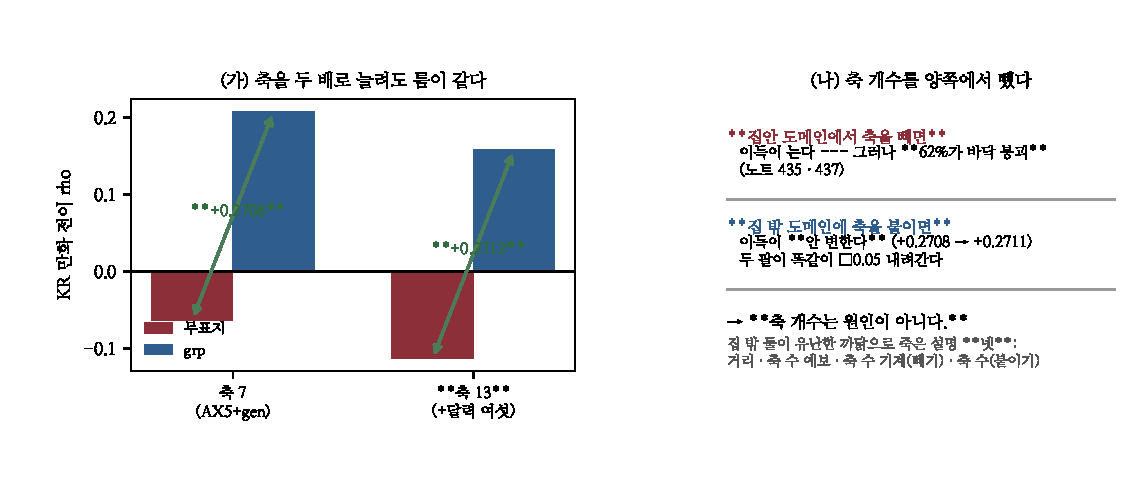
\includegraphics[width=\textwidth]{figs/fig438.pdf}
\caption{(가) 축을 $7 \to 13$ 으로 늘려도 두 팔 사이 틈이 같다.
(나) 축 개수를 빼기와 붙이기 양쪽에서 배제한다.}
\end{figure}

\end{document}
